\chapter{Redes parenclíticas}\label{cap:redes_parencliticas}

En el capítulo anterior hemos visto una serie de algoritmos de machine learning clásicos como lo son los árboles de decisión, las redes neuronales y los Support Vector Machine. En este capítulo veremos un nuevo método basado en teoría de grafos para el problema de clasificación: las redes parenclíticas.\\

Este nuevo método se ha utilizado con éxito en la clasificación de sujetos con glomerolunefritis~\cite{metabo3010155, 1304.1896} (enfermedad renal en la que se daña el sector de los riñones que ayuda a filtrar los desechos y los líquidos de la sangre), con magníficos resultados, llegando a clasificar al 100\% de los sujetos con esta enfermedad. Además, se señala que este método es menos sensible ruido que otros algoritmos clásicos de machine learning como el perceptrón multicapa, los árboles de decisión o Naïve Bayes~\cite{metabo3010155}. En~\cite{Zanin2014} se aplican las redes parenclíticas a los genes de la planta \textit{Arabidopsis thaliana}. Este método permitió el descubrimiento de nuevos genes involucrados en respuestas a estrés osmótico. En~\cite{Zanin2012} se usan las redes parenclíticas para la optimización de series temporales multivariantes. En~\cite{1506.04421} se utilizan redes parenclíticas para la clasificación de los datos de metilación del ADN humano. Aplicado en 14 distintos tipos de cáncer, en 12 de ellos se obtiene una gran tasa de clasificación (clasificando como paciente con cáncer o sin cáncer), situándose en torno al 90--100\%.\\

El método de redes parenclíticas se puede representar de forma sintética en la Figura~\ref{fig:redesparencliticas}. Partiendo de unos datos estructurados (datos que constan de un número fijo de características o variables, representados normalmente en una matriz: cada una de las filas es una observación y las columnas son cada de las variables), se calcula la curva de regresión sobre cada par de variables, y se calcula el error de la estimación obtenida sobre un nuevo ejemplo (que no ha sido ajustado el modelo de regresión con él), que será el peso de la arista de entre las dos variables en el grafo. Con todas las redes parenclíticas (cada una de ellas asociada a una observación cuyos nodos corresponden a las variables) se obtienen distintas medidas, que se pasan a un algoritmo de machine learning clásico, que obtiene la clasificación final.     

\begin{figure}[htbp!]
	\begin{center}
		\resizebox{\textwidth}{!}{%
			\redesparencliticas
		}
	\end{center}
	\caption{Esquema de redes parenclíticas}
	\label{fig:redesparencliticas}
\end{figure}

En este capítulo veremos una introducción a la teoría de grafos, y veremos cómo pasar de la teoría de grafos a las redes complejas, y por último veremos en qué consiste el método de redes parenclíticas.

\section{Introducción a la teoría de grafos}

La teoría de grafos es la rama de las matemáticas que estudia los grafos, objetos matemáticos que constan de dos elementos: los nodos o vértices y las aristas~\cite{opac-b1093081}.\\

La teoría de grafos se inicia con un artículo de Leonhard Euler publicado en 1736 donde resolvía el problema de los puentes de Königsberg~\cite{Euler1736}. La ciudad de Königsberg es atravesada por el río Pregel, que se bifurca en dos para dividir la ciudad en cuatro zonas distintas, que estaban conectadas por siete puentes (Figura~\ref{fig:bridges}).\\

\begin{figure}[htbp!]
\centering
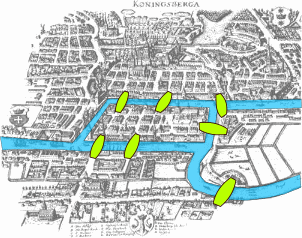
\includegraphics[width=0.6\linewidth]{imagenes/bridges}
\caption{Situación de los siete puentes sobre la ciudad de Königsberg}
\label{fig:bridges}
\end{figure}

El problema consistía en encontrar un camino que recorriera la ciudad, pasando por cada puentes una única vez y regresara al punto de inicio. Euler probó que este problema no tiene solución, por lo que no es posible recorrer los siete puentes y volver al punto inicial, empleando un nuevo concepto: los grafos.\\

A continuación, introduciremos el concepto de grafo, algunas operaciones que se pueden realizar con ellos y alguna de las medidas sobre grafos que utilizaremos a lo largo de la memoria.\\

\begin{defi}
	Un grafo (o grafo no dirigido) es un par $G = (V,E)$ de conjuntos que satisfacen que $E \subseteq V^2$ y $V \cap E = \emptyset$. Los elementos de $V$ se denominan vértices (o nodos) del grafo $G$ y los elementos de $E$ se denominan arcos (o aristas). Una arista entre los vértices $x, y \in V$ se denota como $xy$ o $yx \in E$.
\end{defi}

La forma usual de representar un grafo es dibujar un punto (o círculo) por cada vértice y unir dos de estos dos puntos (o círculos) con una línea para formar un arco. Cómo estén dibujados los vértices y los arcos es irrelevante, sólo importa qué pares de nodos forman una arista y cuáles no.

\begin{ejemplo}
	
	La Figura~\ref{fig:grafo} muestra la representación gráfica de un grafo. Matemáticamente, el grafo es el par $(V, E)$ donde
	
	\[ V = \{A, B, C, D\} \]
	\[ E = \{\{A,B\},\{A,C\},\{B,C\},\{C,D\} \} \]
	
	\begin{figure}[htb]
		\centering
		\ejemplografo
		\caption{Ejemplo de grafo}
		\label{fig:grafo}
	\end{figure}
	
\end{ejemplo}

\begin{defi}
	Se llama orden de un grafo $G$ al número de vértices de dicho grafo. Se denota como $|G|$.\\
	Un grafo $G$ se dice que es finito si $|G| < \infty$. Si $|G| = \infty$ se dice que el grafo $G$ es infinito.
\end{defi}

\begin{ejemplo}
	El grafo de la Figura~\ref{fig:grafo} es un grafo finito, puesto que el número de vértices del grafo es $4$.
\end{ejemplo}

En esta memoria trabajaremos sólo con grafos finitos.

\begin{defi}
	Dos vértices $x,y \in V$ del grafo $G = (V,E)$ se dicen adyacentes si existe una arista entre $x$ e $y$ (o $xy \in E$).
\end{defi}

\begin{defi}\label{def:completo}
	Un grafo se dice completo si todos sus vértices son adyacentes.
\end{defi}

\begin{ejemplo}
	El grafo de la Figura~\ref{fig:grafo_completo} es completo ya que todos sus vértices son adyacentes. En efecto, el vértice $A$ tiene una arista que lo une con los nodos $B$, $C$ y $D$. De la misma forma, se comprueba para los vértices $B$, $C$ y $D$.
	
	\begin{figure}[htb]
		\centering
		\ejemplografocompleto
		\caption{Ejemplo de grafo completo}
		\label{fig:grafo_completo}
	\end{figure}
	
\end{ejemplo}

\begin{defi}
	Un grafo dirigido (o digrafo) es un par $(V,E)$ de conjuntos disjuntos (de vértices y de aristas) junto con dos funciones $\mathrm{init} : E \to V$ y $\mathrm{ter} : E \to V$ que asigna a cada arista $e$ un vértice inicial $\mathrm{init}(e)$ y un vértice terminal $\mathrm{ter}(e)$.\\
	
	La arista $e$ se dice dirigida desde $\mathrm{init}(e)$ hasta $\mathrm{ter}(e)$.\\
	
	Si $\mathrm{init}(e) = \mathrm{ter}(e)$, la arista $e$ se dice que es un bucle.
\end{defi}

\begin{ejemplo}
	La Figura~\ref{fig:grafo_dirigido} muestra la representación gráfica un grafo dirigido. Matemáticamente, es el par $(V,E)$ donde
	
	\[V  = \{A, B, C, D\}\]
	\[E = \{ \{A,B\}, \{A,C\}, \{C,C\},\{B,C\}, \{C,D\} \} \]
	
	junto con las funciones $\mathrm{init} : E \to V $ y $\mathrm{ter} : E \to V$ definidas de la siguiente manera:
	
	\begin{center}
		\begin{tabular}{l|r}
			\begin{tabular}{r c c c}
				$\mathrm{init}:$ & $E$ & $\to$ & $V$\\
				& $\{A,B\}$ & $\mapsto$ & $A$\\
				& $\{A,C\}$ & $\mapsto$ & $A$\\
				& $\{C,C\}$ & $\mapsto$ & $C$\\
				& $\{B,C\}$ & $\mapsto$ & $B$\\
				& $\{C,D\}$ & $\mapsto$ & $C$\\
				
			\end{tabular} &
			\begin{tabular}{r c c c}
				$\mathrm{ter}:$ & $E$ & $\to$ & $V$\\
				& $\{A,B\}$ & $\mapsto$ & $B$\\
				& $\{A,C\}$ & $\mapsto$ & $C$\\
				& $\{C,C\}$ & $\mapsto$ & $C$\\
				& $\{B,C\}$ & $\mapsto$ & $C$\\
				& $\{C,D\}$ & $\mapsto$ & $D$\\
				
			\end{tabular} 
		\end{tabular}
	\end{center}
	
	Además la arista $\{C,C\}$ es un bucle porque $\mathrm{init}(\{C,C\}) = \mathrm{ter}(\{C,C\}) = C$.
	
	\begin{figure}[h]
		\centering
		\ejemplografodirigido
		\caption{Ejemplo de grafo dirigido con bucle}
		\label{fig:grafo_dirigido}
	\end{figure}
	
\end{ejemplo}

\begin{defi}
	Un grafo ponderado o pesado es un grafo con una función $\mathrm{w} : E \to \R$, es decir, que $\mathrm{w}$ asocia un número real a cada arista. Esta función recibe el nombre de función peso.
\end{defi}

\begin{ejemplo}
	El grafo $G = (V,E)$ con 
	
	\begin{eqnarray}
	V = \{A, B, C\}\\
	E = \{ \{A,B\}, \{A,C\}, \{B,C\} \}
	\end{eqnarray} 
	
	es un grafo. Si le añadimos la función $\mathrm{w} : E \to \R$ definida de la siguiente forma, $G$ es un grafo ponderado (ver Figura~\ref{fig:grafo_ponderado}).
	
	\begin{equation*}
	\begin{tabular}{r c c c}
	$\mathrm{w}:$ & $E$ & $\to$ & $\R$\\
	& $\{A,B\}$ & $\mapsto$ & $e$\\
	& $\{A,C\}$ & $\mapsto$ & $5$\\
	& $\{B,C\}$ & $\mapsto$ & $\pi$
	
	\end{tabular}
	\end{equation*}
	\begin{figure}[htb]
		\centering
		\ejemplografoponderado
		\caption{Ejemplo de grafo ponderado}
		\label{fig:grafo_ponderado}
	\end{figure} 
\end{ejemplo}

\begin{defi}
	Dado un grafo ponderado $G = (V,E)$ y $\mathrm{w} : E \to \R$, decimos que una arista $e \in E$ incide en el vértice $v \in V$, si $\mathrm{ter}(e) = v$. 
\end{defi}

\begin{defi}
	La fuerza de un vértice en un grafo ponderado se define como la suma de todos los pesos de sus aristas incidentes.
\end{defi}

\subsection{Algunas medidas}\label{sec:medidas}

\begin{defi}
	Se define densidad de enlaces\footnote{Traducción de link density} del grafo $G$ como el número de enlaces dividido entre el número de enlaces que pueden estar presentes en el grafo.
	\begin{equation}\label{eq:densidad}
	d(G) = \dfrac{1}{n(n-1)} \sum_{i,j} a_{i,j}
	\end{equation}
	
	donde $n$ es el número de nodos del grafo y $a_{i,j}$ es la entrada ij-ésima de la matriz de adyacencia (matriz que en su posición $(i,j)$ indica si existe una arista entre el nodo $i$ y $j$).
\end{defi}

\begin{defi}
	Se define coeficiente de clustering $C$ del grafo $G$ como
	
	\begin{equation}\label{eq:clustering}
	C(G) = \dfrac{3N_{\triangle}}{N_3}
	\end{equation}
	
	donde $N_{\triangle}$ es el número de triángulos del grafo y $N_3$ es el número de tripletas conectadas.
\end{defi}

\begin{defi}
	Se define eficiencia de un grafo $G$ como
	
	\begin{equation}\label{eq:eficiencia}
	\mathrm{E}(\mathcal{G}) = \dfrac{1}{\binom{n}{2}} \sum_{i\neq j} \dfrac{1}{d(i,j)}
	\end{equation}
	
	donde $d(i,j)$ es la distancia entre el nodo $i$ y el nodo $j$ y $n$ es el número de nodos de $G$.
\end{defi}

La eficiencia es la media armónica de todos los caminos del grafo de competitividad.\\

Para calcular la distancia entre los nodos del grafo se pueden aplicar los algoritmos de Dijkstra o Floyd (Ver~\cite{Cormen:2001:IA:580470}).

\begin{defi}
	Se define longitud del camino característico\footnote{Traducción de characteristic path length} del grafo $G$ de la siguiente forma:
	
	\begin{equation}\label{eq:camino}
	\mathrm{L}(\mathcal{G}) = \dfrac{1}{\binom{n}{2}} \sum_{i\neq j} d(i,j)
	\end{equation}
	
	donde $d(i,j)$ es la distancia entre el nodo $i$ y el nodo $j$ y $n$ es el número de nodos de $G$.
\end{defi}

La longitud del camino característico es la media aritmética de todos los caminos del grafo.\\

En~\cite{cond-mat/0505185} se pueden encontrar una extensa lista con distintas medidas sobre grafos. 


\section{De la teoría de grafos a las redes parenclíticas}

A continuación describimos el método de redes parenclíticas propuesto en~\cite{metabo3010155}.\\

Supongamos que tenemos un conjunto de datos con $n$ variables para cada una de las $m$ observaciones, y cada una de éstas vienen clasificadas en la clase $c$ o $d$. Estas dos clases actuarán como datos de entrenamiento. Además, se supone que existe una observación, que llamaremos X, para la que la clase se desconoce.\\

El objetivo es construir un grafo, extraer de una serie de medidas y conseguir su clasificación mediante algoritmos clásicos de machine learning.\\

La creación del grafo requiere analizar todos los pares de nodos. Para ello, se proyectan cada par de variables sobre el plano xy y se aplica un modelo. En~\cite{metabo3010155, 1304.1896, Zanin2014} se aplican modelos de regresión lineal.

\begin{equation}
y = \alpha_1 x + \alpha_2 + \varepsilon
\end{equation} 

donde $\alpha_1$ es la pendiente del modelo, $\alpha_2$ es el término independiente y $\varepsilon$ es el término del error del modelo.\\

Esto se hace por cada clase, dando lugar a dos modelos distintos. Se puede representar la salida de la variable proyecta de la observación $X$ como dos distribuciones normales (una por cada clase) con parámetros $\mu$ como el valor esperado de la variable salida y $\sigma$ como la desviación estándar del vector $\epsilon$.\\

Se puede asignar una probabilidad a cada una de las clases de la siguiente forma.

\begin{equation}\label{eq:prob1}
p_d = \dfrac{\tilde{p}_d}{\tilde{p}_d + \tilde{p}_c}
\end{equation}

\begin{equation}\label{eq:prob2}
p_c = \dfrac{\tilde{p}_c}{\tilde{p}_d + \tilde{p}_c}
\end{equation}

donde $\tilde{p}_d$, $\tilde{p}_d$ son las probabilidades de estar en la clase $d$ o $c$ dadas por las distribuciones normales mencionadas anteriormente.\\

Para formar el grafo, asociamos un peso a la arista entre esas dos variables dado por el error entre el valor estimado y el valor real, es decir,

\begin{equation}
\hat{\varepsilon} = |\hat{y} - y|,
\end{equation} 

donde $\hat{y}$ es el valor estimado y $y$ es el valor real de la variable salida, de la clase con mayor probabilidad de las calculadas anteriormente.\\

\begin{ejemplo}
	Supongamos que disponemos de los datos de la Tabla~\ref{tbl:ejemploredparenclitica}, y queremos construir la red parenclítica del individuo $X = (3,3)$, y obtener su clasificación.\\
	
	\begin{table}[htbp!]
		\centering
		\caption{Datos del ejemplo}
		\label{tbl:ejemploredparenclitica}
		\begin{tabular}{@{}ccc@{}}
			\toprule
			x    & y   & Clase \\ \midrule
			0.5  & 1.5 & A     \\
			1.5  & 2.5 & A     \\
			1.2  & 2.5 & A     \\
			0.75 & 2   & A     \\
			0.6  & 1.9 & A     \\
			0.77 & 2.5 & A     \\
			1.5  & 3   & A     \\
			1.3  & 3.3 & A     \\
			0.6  & 3.2 & A     \\
			4    & 1   & B     \\
			3.3  & 0.3 & B     \\
			4.5  & 1.2 & B     \\
			4.5  & 0.5 & B     \\
			3.9  & 0.7 & B     \\
			5    & 1   & B     \\
			3.5  & 0.2 & B     \\
			4    & 0.3 & B     \\ \bottomrule
		\end{tabular}
	\end{table}
	
	En primer lugar calculamos la rectas de regresión de cada una de las clases A y B (Figura~\ref{fig:reg_rectas}).\\
	
	\begin{figure}[htbp!]
		\centering
		\regresionred
		\caption[Recta de regresión de cada una de las clases]{Recta de regresión de cada una de las clases. La clase A se muestra en azul y la clase B en naranja}
		\label{fig:reg_rectas}
	\end{figure}
	
	Las rectas para las clases A y B son respectivamente:
	
	\begin{align*}
	y_A & = 0.82x + 1.69, \\
	y_B & = 0.46x - 1.25,
	\end{align*}
	
	y las desviaciones típicas de los residuos son:
	
	\begin{align*}
	\sigma_A & = 0.5135,\\
	\sigma_B & = 0.2801
	\end{align*}
	
	Por tanto, imponemos que la probabilidad de estar en cada una de las clases es una variable aleatoria normal con media, el valor esperado de $x$ sobre la recta de regresión del individuo $X$, y desviación típica, la obtenida de los residuos del modelo:
	
	\begin{align*}
	Y_A & = \mathcal{N}(0.82\cdot 3 + 1.69, 0.5135) = \mathcal{N}(4.15, 0.5135)\\
	Y_B & = \mathcal{N}(0.46\cdot 3 - 1.25, 0.2801) = \mathcal{N}(0.13, 0.2801)
	\end{align*}
	
	La Figura~\ref{fig:dist_normales} muestra este hecho. Por tanto, la probabilidad de estar en cada una de las clase viene dado por 
	
	\begin{figure}[htbp!]
		\centering
		\distnormales
		\caption{Distribuciones normales}
		\label{fig:dist_normales}
	\end{figure}
	
	\begin{align*}
	\tilde{p}_A & = \dfrac{\tilde{p}_A}{\tilde{p}_A + \tilde{p}_B} = \dfrac{0.063}{0.063 + 0} = 1 \\
	\tilde{p}_B & = \dfrac{\tilde{p}_A}{\tilde{p}_A + \tilde{p}_B} = \dfrac{0}{0.063 + 0} = 0 \\
	\end{align*}
	
	Por tanto, la probabilidad mayor es de que el individuo $X$ que pertenezca a la clase A.\\
	
	Así pues, el error cometido en esta aproximación es
	
	\begin{equation*}
	\epsilon = |4.15 - 3| = 1.15
	\end{equation*}
	
	Éste es el peso entre los nodos $x$,$y$, que da lugar a la red parenclítica del individuo $X$ (Figura~\ref{fig:red_par}).\\
	
	\begin{figure}[htbp!]
		\centering
		\ejemploredparenclitica
		\caption{Red parenclítica del ejemplo}
		\label{fig:red_par}
	\end{figure}
	
	En caso de tener más variables repetiríamos este proceso con cada par de variables. Una vez obtenidas todas las redes parenclíticas de los individuos desconocidos, se extraerían medidas de los grafos como las vistas en la Sección~\ref{sec:medidas}, que actuarían como entrada a un algoritmo de machine learning visto en la Sección~\ref{cap:ml}, que obtendría la clasificación. 
\end{ejemplo}

Este método tiene algunas limitaciones:

\begin{enumerate}
	\item Las variables no tienen por qué comportarse de forma lineal, por lo que este modelo podría ajustar de forma incorrecta.
	\item Se limita a una clasificación binaria. 
\end{enumerate}

La primera limitación se puede solventar aplicando otros métodos distintos al lineal.\\

Proponemos aplicar tres métodos distintos:

\begin{enumerate}
	\item Exponencial
	
	\begin{equation}
	y = \exp(\alpha_1 + \alpha_2 x) \quad \alpha_1, \alpha_2 \in \R
	\end{equation}
	
	\item Cuadrático
	
	\begin{equation}
	y = (\alpha_1 + \alpha_2 x)^2 \quad \alpha_1, \alpha_2 \in \R
	\end{equation}
	
	\item Recíproco
	
	\begin{equation}
	y = \dfrac{1}{\alpha_1 + \alpha_2 x} \quad \alpha_1, \alpha_2 \in \R
	\end{equation}
\end{enumerate}

Estos métodos pueden ser linealizados como hemos visto en la Tabla~\ref{tbl:linealizacion}.\\

La segunda limitación se puede solventar generalizando la Fórmula~\ref{eq:prob1} a lo siguiente:

\begin{equation}
p_i = \dfrac{\tilde{p}_i}{\displaystyle \sum_{i} \tilde{p}_i }
\end{equation}

donde ${p}_i$ es la probabilidad de pertenecer a la clase $i$.\\

Una vez hecho ésto se puede aplicar el método descrito. Seguimos suponiendo normalidad de las variables.\\

En el capítulo siguiente veremos el diseño y la tecnología utilizada para implementar una aplicación que permita analizar un conjunto de datos utilizando las redes parenclíticas.